


\section{Other implied changes to the current operations proposal}
Notably missing from \figref{fig:sciopsorg} is \gls{QA}. Currently \gls{QA} is spread across  three
 departments - the suggestion here is to place all \gls{QA} activities under the survey performance department. Consolidation
of the \gls{QA} activities in one department may allow for some personnel saving.

The data release team in science operations would require a verification scientist (this may be 0.5FTE) while the \gls{SDQA} and Semantic scientists may move to QA in survey science.

All data facility work, be it with a partner or in commercial \gls{cloud} should be firmly under science operations - hence there is no LDF department and no associate director for LDF as depicted in \figref{fig:opsorg}.\footnote{This is  in line with AMCL recommendations}


\begin{figure}
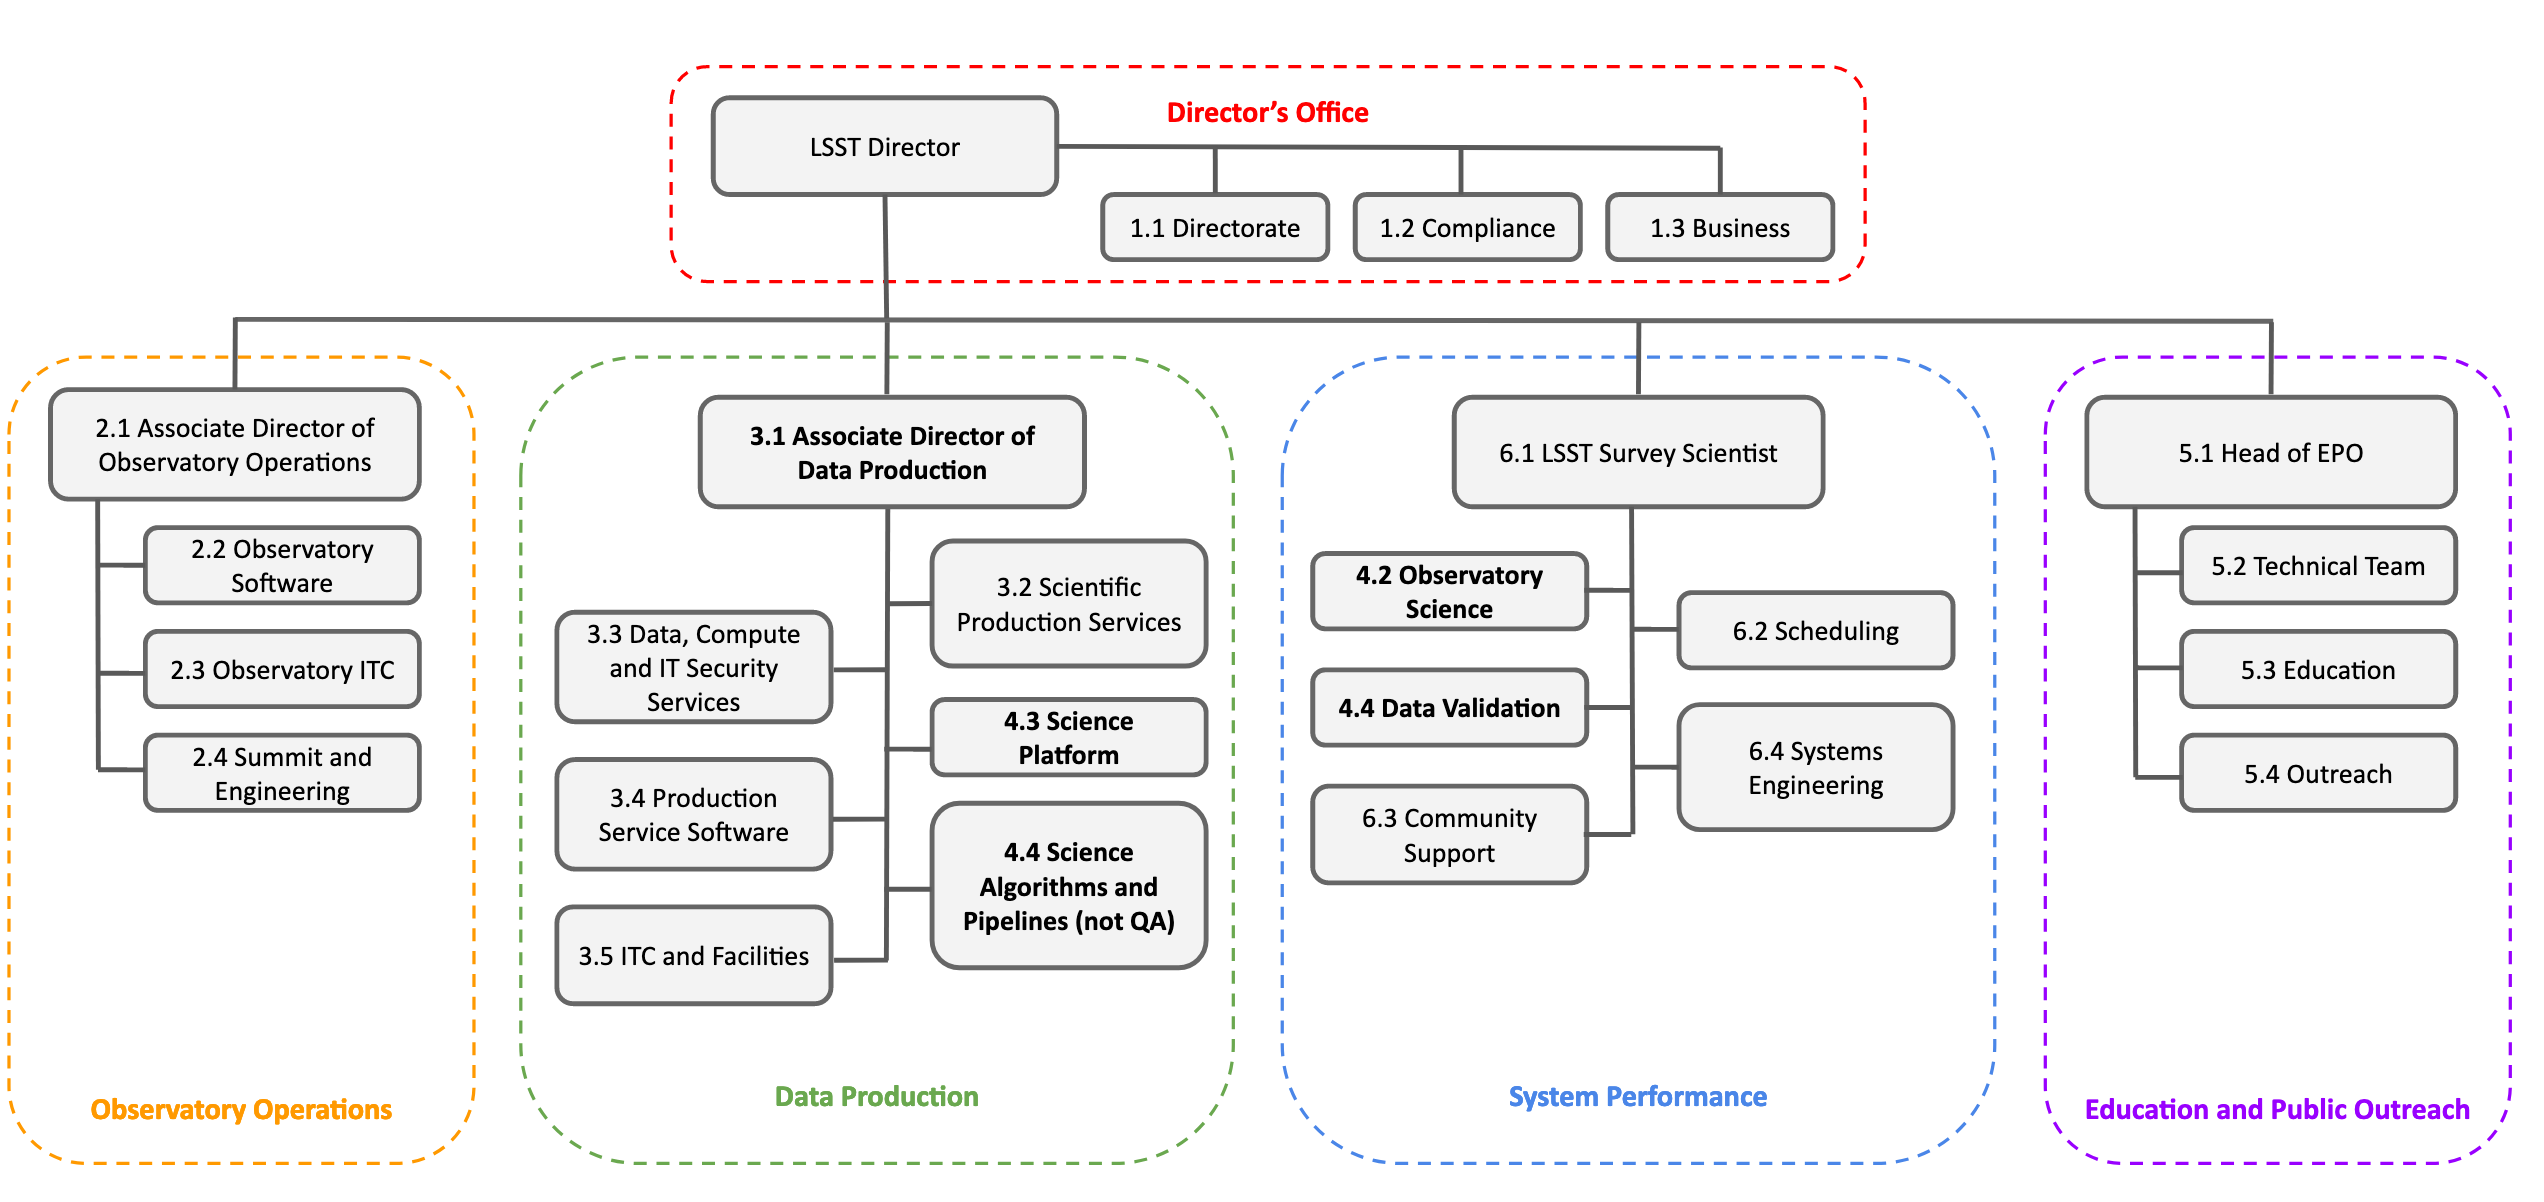
\includegraphics[width=1.0\textwidth]{figures/OpsOrg}
\caption{Possible new organisation chart for \gls{LSST}  operations \label{fig:opsorg}}
% original https://docs.google.com/presentation/d/1H7sn92FXDa9-cgFrizgN12KI3Br60Ffbk4qA8fxCvMg/edit#slide=id.g5132af8469_0_81
\end{figure}

\textbf{NOTE: I have said before communications should report directly to the director - in \figref{fig:opsorg} there is NO communications.}

ITC and facilities (\figref{fig:opsorg}) in this model should come from \gls{NCOA}  logically also this does not belong in data production but at a higher level its for the entire org, the observatory already has its own \gls{ITC} group so they are good.


There are still some developments in \gls{NCSA} such as \gls{DAQ} forwarders which would need to be included in possibly the observatory \gls{software}.

There are other developments \gls{DBB} which could be replaced by commodity services like Amazon \gls{S3} which includes replications and reliability.
